\documentclass{beamer}
\usepackage{graphics,amssymb,amsfonts,amsmath}
\usepackage{pgf,tikz}
\usetikzlibrary{shapes,shapes.geometric,positioning,trees}
\DeclareGraphicsExtensions{.jpg,.pdf,.mps,.png}
\usepackage[utf8]{inputenc}
\usepackage[brazil]{babel}
\usepackage[normalem]{ulem}
\usepackage{standalone}
\usepackage{pgfpages,enumerate,hyperref}
\usepackage{palatino}   %Fonte sem serifa.
\usepackage{ragged2e}   %Par\'agrafo justificado.
\usepackage{minted}
\usepackage{tikz}
% \usetheme{CambridgeUS}
% \usetheme{AnnArbor}
% \usecolortheme{lily}
\usecolortheme{orchid}
\usefonttheme[onlymath]{serif}

\def\theFancyVerbLine{%
  \rmfamily\tiny\arabic{FancyVerbLine}%
  {\tikz[remember picture,overlay]\node(minted-\arabic{FancyVerbLine}){};}%
}

%colocando n\'umero de p\'aginas no slide.
\setbeamertemplate{footline}[frame number]

% desativando os botoes de navegacao.
\beamertemplatenavigationsymbolsempty

%Tela cheia
\hypersetup{pdfpagemode=FullScreen}

% Layout da p\'agina
\hypersetup{pdfpagelayout=SinglePage,urlcolor=blue,colorlinks=true}

% Ambiente bash
\newminted{bash}{bgcolor=black,formatcom=\color{white}}

% Ambiente python
\newminted{python}{bgcolor=green!25!white,linenos}

% Ambiente html
\newminted{html}{bgcolor=cyan!25}

\tikzstyle{every node}=[anchor=west]
\tikzstyle{selected}=[draw=red,fill=green!30]
\tikzstyle{optional}=[dashed,fill=gray!50]

\title{Tutorial Django - Parte 2\\ Django ORM and Fixtures}
\author{R\'egis da Silva\\ {\texorpdfstring{\color{blue}}{ }about.me/rg3915}}
\institute{\url{github.com/grupy-sp/encontros}}
\date{24 de Outubro de 2015}

\begin{document}
\justifying %Par\'agrafo justificado.

%Neste caso insere somente no primeiro slide.
{%
%\usebackgroundtemplate{\centering \vspace*{5cm} \includegraphics[width=\paperwidth]{figuras/djangoPython}}

% \usebackgroundtemplate{%
% \vbox to \paperheight{\vfil\hbox to \paperwidth{\hfil\includegraphics[width=\paperwidth]{img/logo_mascote.jpg}\hfil}\vfil}
% }

% \begin{frame}

% \end{frame}
% }

\begin{frame}
	\titlepage
\end{frame}

\begin{frame}[fragile]\frametitle{Livraria}
	
\textbf{Tema}: Modelagem de banco de dados de uma \textbf{livraria}.

\

Começando...

\begin{bashcode}
	$ git clone https://github.com/rg3915/
      django-orm.git
	$ virtualenv -p python3 django-orm
	$ cd django-orm
	$ source bin/activate
	$ make initial
	$ make fixtures
	$ ./manage.py runserver
\end{bashcode}

\end{frame}

\begin{frame}\frametitle{Ementa}

\begin{itemize}
	\item Modelagem
	\begin{itemize}
		\item OneToMany
		\item OneToOne
		\item ManyToMany
		\item Abstract Inheritance
		\item Multi-table Inheritance
	\end{itemize}
	\item Fixtures
	\begin{itemize}
		\item random values
		\item csv
		\item shell do Django
	\end{itemize}
	\item Conclusão
\end{itemize}
	
\end{frame}



\begin{frame}\frametitle{Objetivo}
	\begin{itemize}
		\item Criar vários modelos de dados
		\item Popular o banco de dados
	\end{itemize}
\end{frame}

\begin{frame}\frametitle{OneToMany (um para muitos)}
	

É o relacionamento onde usamos \textbf{chave estrangeira},

conhecido como \textbf{ForeignKey}.

	\begin{figure}[h]
	  \centering
  		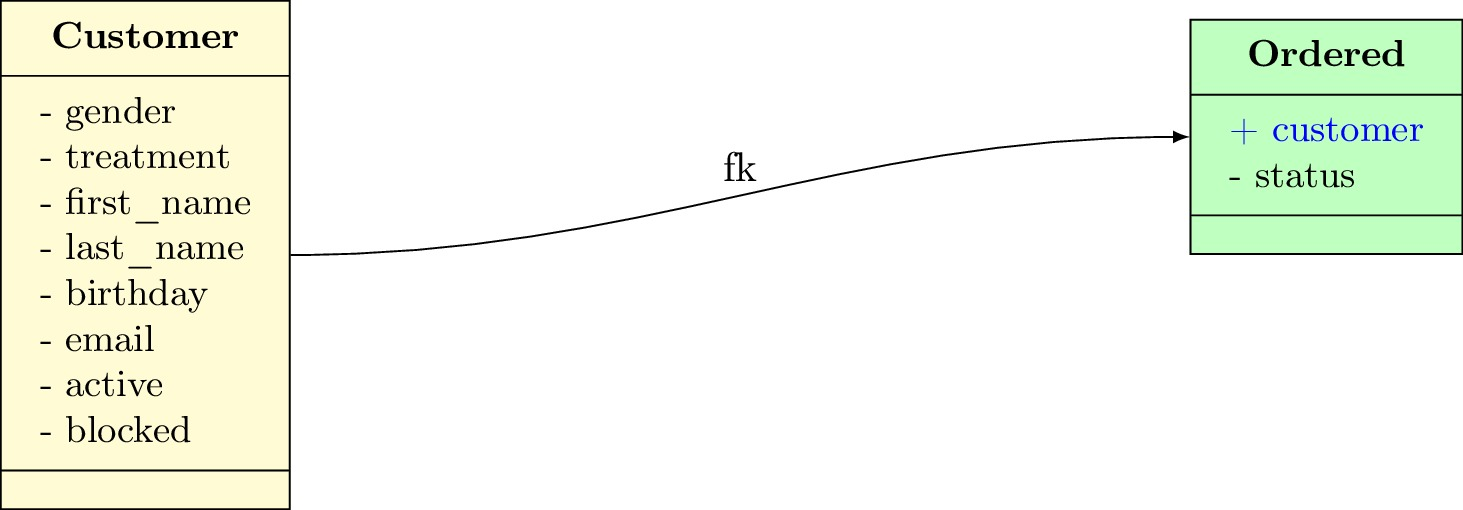
\includegraphics[width=.8\paperwidth]{img/01fk.jpg}
	\end{figure}

Um \textbf{cliente} pode fazer vários \textbf{pedidos}, então para reproduzir o esquema acima, usamos o seguinte código:

\end{frame}

\begin{frame}[fragile]

\begin{pythoncode}
class Customer(models.Model):
    gender = models.CharField(_(u'gênero'), max_length=1, choices=gender_list)
    treatment = models.CharField(
        _('tratamento'), max_length=4, choices=treatment_list, blank=True)
    first_name = models.CharField(_('nome'), max_length=30)
    last_name = models.CharField(_('sobrenome'), max_length=30)
    birthday = models.DateTimeField(_('nascimento'), null=True, blank=True)
    email = models.EmailField(_('e-mail'), blank=True)
    active = models.BooleanField(_('ativo'), default=True)
    blocked = models.BooleanField(_('bloqueado'), default=False)


class Ordered(TimeStampedModel):
    customer = models.ForeignKey(
        'Customer', verbose_name=_('cliente'), related_name='cliente_pedido')
    status = models.CharField(
        _('status'), max_length=2, choices=status_list, default='pe')

\end{pythoncode}


\tikz[remember picture,overlay]\draw[fill=yellow,opacity=0.2] ([yshift=-0.05cm,xshift=14em]minted-14) rectangle ([yshift=0.35cm,xshift=20em]minted-14);

\end{frame}

\begin{frame}\frametitle{OneToOne (um para um)}
Neste tipo de relacionamento também usamos \textbf{chave estrangeira}, só que um registro de uma tabela se relaciona apenas com um registro da outra tabela.

	\begin{figure}[h]
	  \centering
  		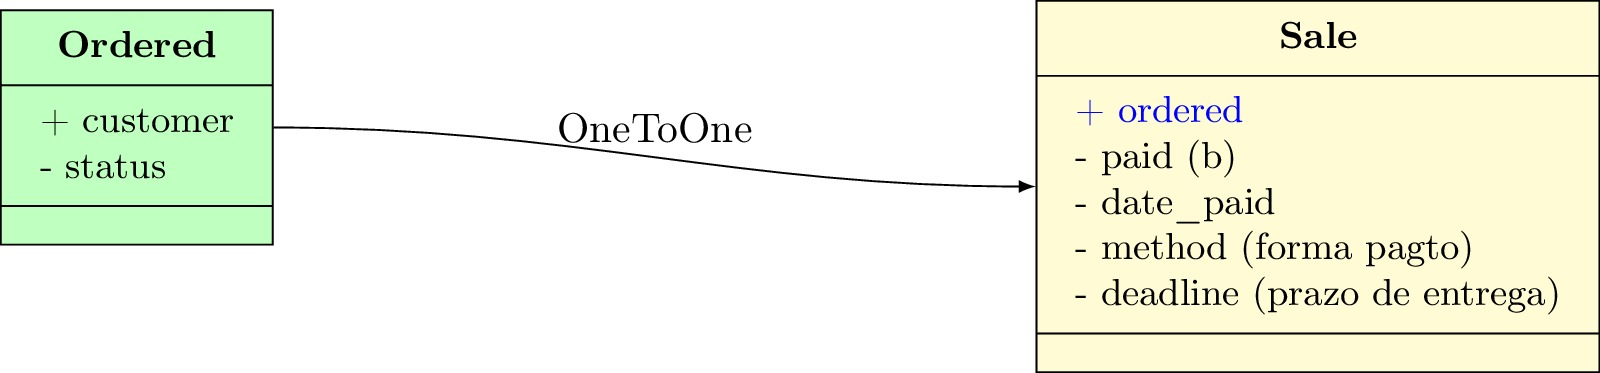
\includegraphics[width=.8\paperwidth]{img/02oneToone.jpg}
	\end{figure}

Uma \textbf{venda} pode ser feita a partir de apenas um \textbf{pedido}, então para reproduzir o esquema acima, usamos o seguinte código:
\end{frame}

\begin{frame}[fragile]

\begin{pythoncode}
class Ordered(TimeStampedModel):
    customer = models.ForeignKey(
        'Customer', verbose_name=_('cliente'), related_name='cliente_pedido')
    status = models.CharField(
        _('status'), max_length=2, choices=status_list, default='pe')


class Sale(models.Model):
    ordered = models.OneToOneField('Ordered',
                        verbose_name=_('pedido'))

    paid = models.BooleanField(_('pago'), default=False)
    date_paid = models.DateTimeField(_('pago em'), null=True, blank=True)
    method = models.CharField(_('forma de pagto'), max_length=20, blank=True)
    deadline = models.CharField(
        _('prazo de entrega'), max_length=50, blank=True)

\end{pythoncode}

\end{frame}

\begin{frame}\frametitle{ManyToMany (muitos para muitos)}
	
Este relacionamento permite que vários registros de uma tabela se relacione com vários registros da outra tabela.

	\begin{figure}[h]
	  \centering
  		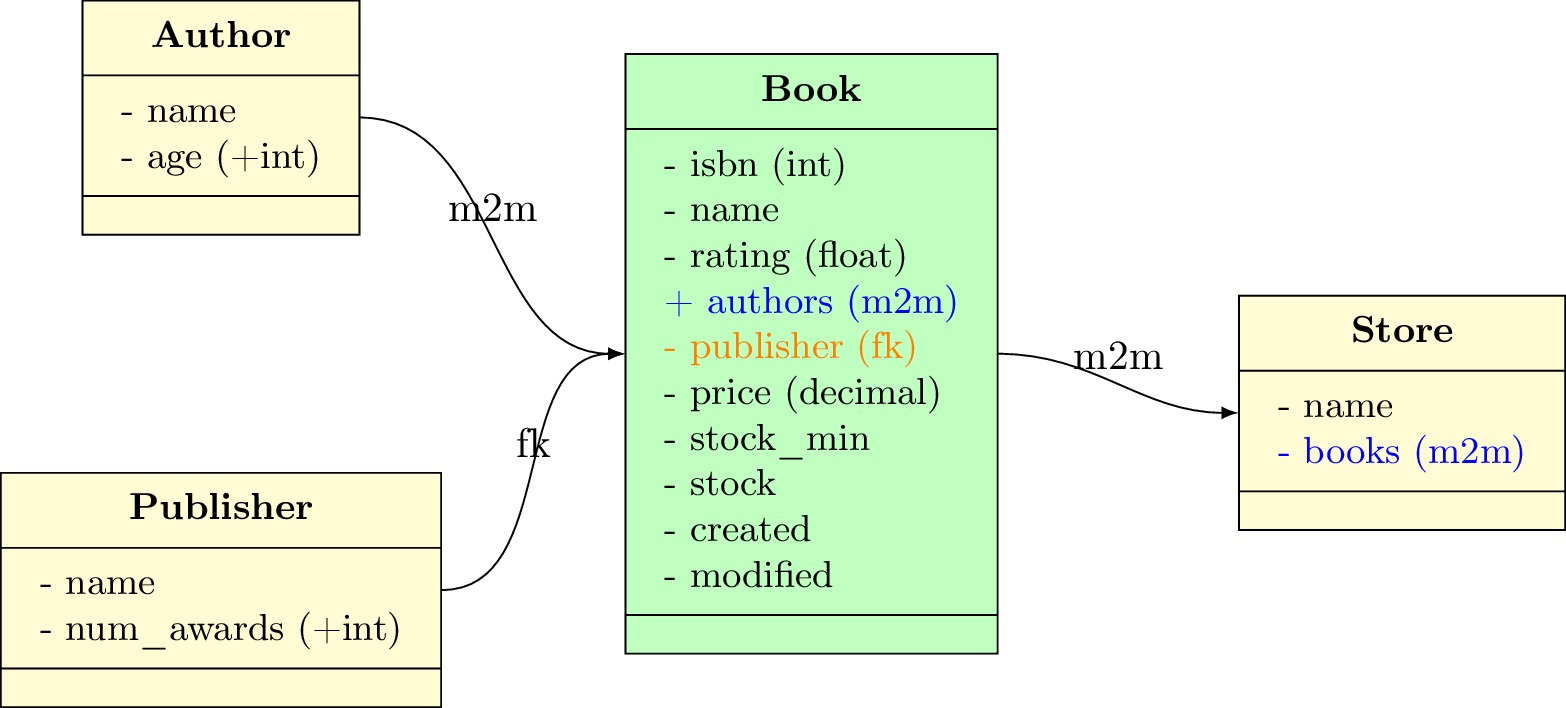
\includegraphics[width=.75\paperwidth]{img/03m2m.jpg}
	\end{figure}

Um \textbf{autor} pode ter vários \textbf{livros} e cada \textbf{livro} pode ter vários \textbf{autores}, então para reproduzir o esquema acima, usamos o seguinte código:
\end{frame}

\begin{frame}[fragile]

\begin{pythoncode}
class Author(models.Model):
    name = models.CharField(_('nome'), max_length=50, unique=True)
    age = models.PositiveIntegerField(_('idade'))


class Book(TimeStampedModel):
    isbn = models.IntegerField()
    name = models.CharField(_('nome'), max_length=50)
    rating = models.FloatField(_(u'classificação'))

    authors = models.ManyToManyField('Author',
                            verbose_name='autores')

    publisher = models.ForeignKey('Publisher', verbose_name='editora')
    price = models.DecimalField(_(u'preço'), max_digits=5, decimal_places=2)
    stock_min = models.PositiveIntegerField(_(u'Estoque mínimo'), default=0)
    stock = models.IntegerField(_('Estoque atual'))
\end{pythoncode}

\end{frame}


\begin{frame}[fragile]
	
E o mesmo para \textbf{lojas}.

\begin{pythoncode}
class Store(models.Model):
    name = models.CharField(_('nome'), max_length=50)
    books = models.ManyToManyField('Book', verbose_name='livros')
\end{pythoncode}

\end{frame}

\begin{frame}
	
Por baixo dos panos o Django cria uma terceira tabela (escondida).

	\begin{figure}[h]
	  \centering
  		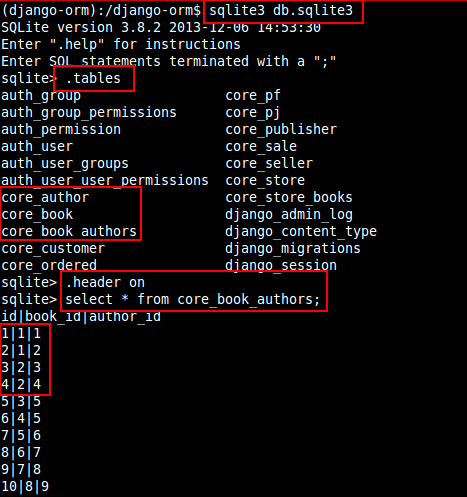
\includegraphics[height=.75\paperheight]{img/sqlite01}
	\end{figure}

Neste caso, temos dois livros com dois autores cada.
\end{frame}

\begin{frame}[fragile]

\begin{bashcode}
id|book_id|author_id
1 |1	  	  |1
2 |1	  	  |2
3 |2	  	  |3
4 |2	  	  |4
\end{bashcode}

\

\


E ainda, na sequência temos dois livros diferentes do mesmo autor.

\begin{bashcode}
id|book_id|author_id
5 |3	  	  |5
6 |4	  	  |5
\end{bashcode}

\end{frame}

\begin{frame}\frametitle{Mais um exemplo}	
Um outro exemplo legal é o caso onde vários \textbf{livros} podem ser entregues por vários \textbf{fornecedores}.

	\begin{figure}[h]
	  \centering
  		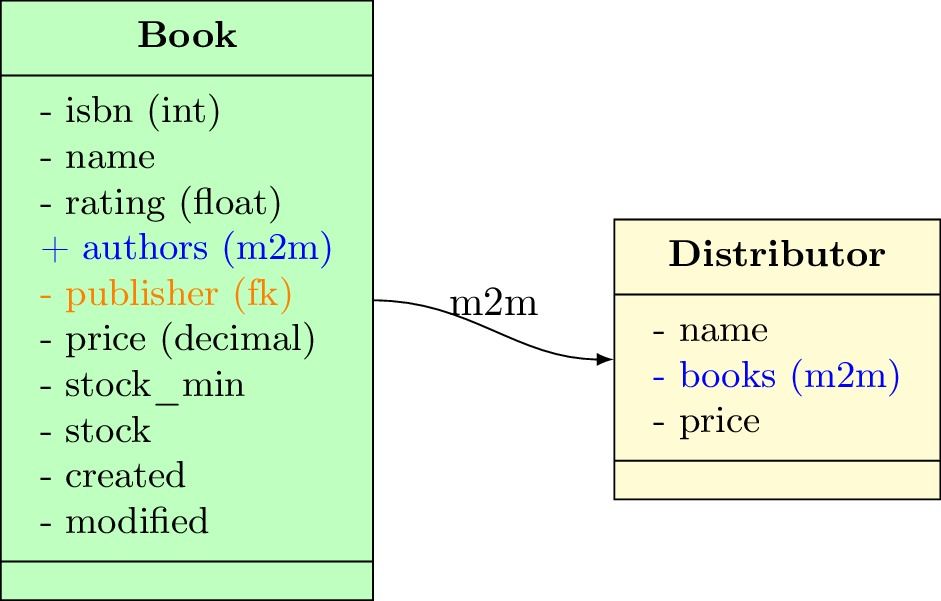
\includegraphics[height=.7\paperheight]{img/04m2m}
	\end{figure}

\end{frame}


\begin{frame}\frametitle{Abstract Inheritance (Herança Abstrata)}

% Neste tipo de modelo o Django cria novas tabelas a partir de uma tabela abstrata (base).

% As novas tabelas são uma **cópia** da primeira.

% Não existe relacionamento entre elas. Mas campos adicionais podem ser criados nas novas tabelas.

	\begin{figure}[h]
	  \centering
  		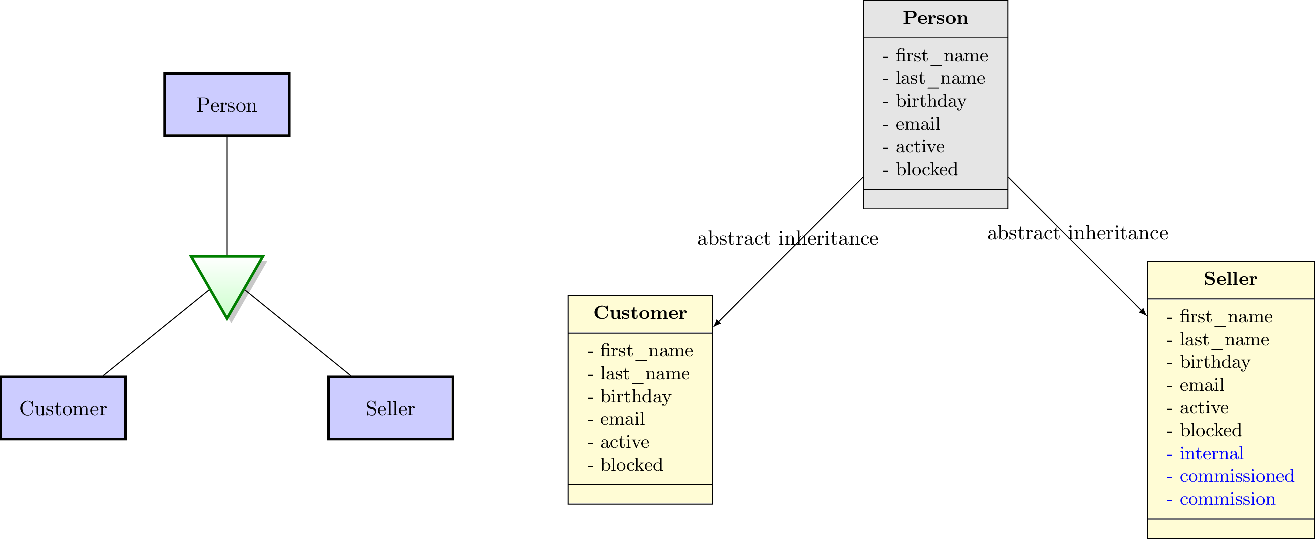
\includegraphics[width=.93\paperwidth]{img/05abstract}
	\end{figure}

\end{frame}

\begin{frame}\frametitle{Abstract Inheritance (Herança Abstrata)}

    \begin{figure}[h]
      \centering
        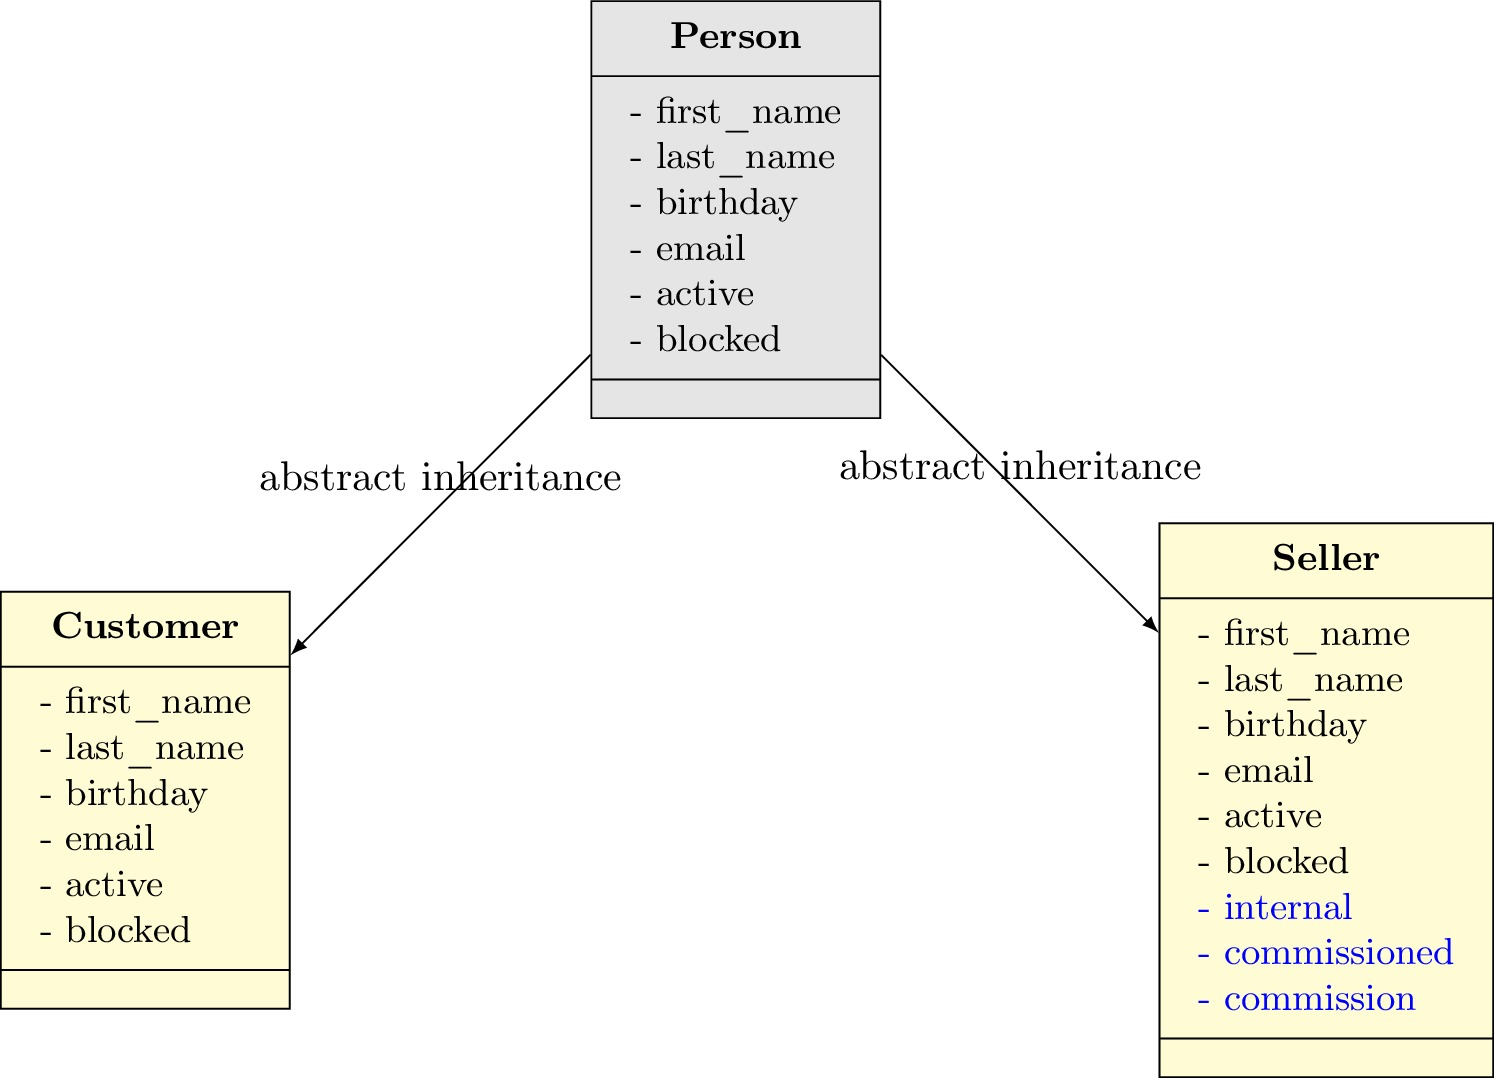
\includegraphics[height=.85\paperheight]{img/051abstract}
    \end{figure}

\end{frame}

\begin{frame}[fragile]
	
\begin{pythoncode}
class Person(models.Model):
    gender = models.CharField(_(u'gênero'), max_length=1, choices=gender_list)
    treatment = models.CharField(
        _('tratamento'), max_length=4, choices=treatment_list, blank=True)
    first_name = models.CharField(_('nome'), max_length=30)
    last_name = models.CharField(_('sobrenome'), max_length=30)
    birthday = models.DateTimeField(_('nascimento'), null=True, blank=True)
    email = models.EmailField(_('e-mail'), blank=True)
    active = models.BooleanField(_('ativo'), default=True)
    blocked = models.BooleanField(_('bloqueado'), default=False)

class Meta:
    abstract = True


class Customer(Person):
    pass
\end{pythoncode}

\end{frame}

\begin{frame}[fragile]

\begin{pythoncode}
class Seller(Person):
    internal = models.BooleanField(_('interno'), default=True)
    commissioned = models.BooleanField(_('comissionado'), default=True)
    commission = models.DecimalField(
        _(u'comissão'), max_digits=6, decimal_places=2, default=0.01, blank=True)
\end{pythoncode}

\

\

Note que a tabela \textbf{Customer} é uma cópia de \textbf{Person}, e \textbf{Seller} também é uma cópia, mas com campos adicionais.
\end{frame}



\begin{frame}\frametitle{Multi-table Inheritance (Herança Multi-tabela)}
    
Na herança múltipla o Django cria um relacionamento \textbf{um pra um (OneToOne)} automaticamente entre as tabelas.

    \begin{figure}[h]
      \centering
        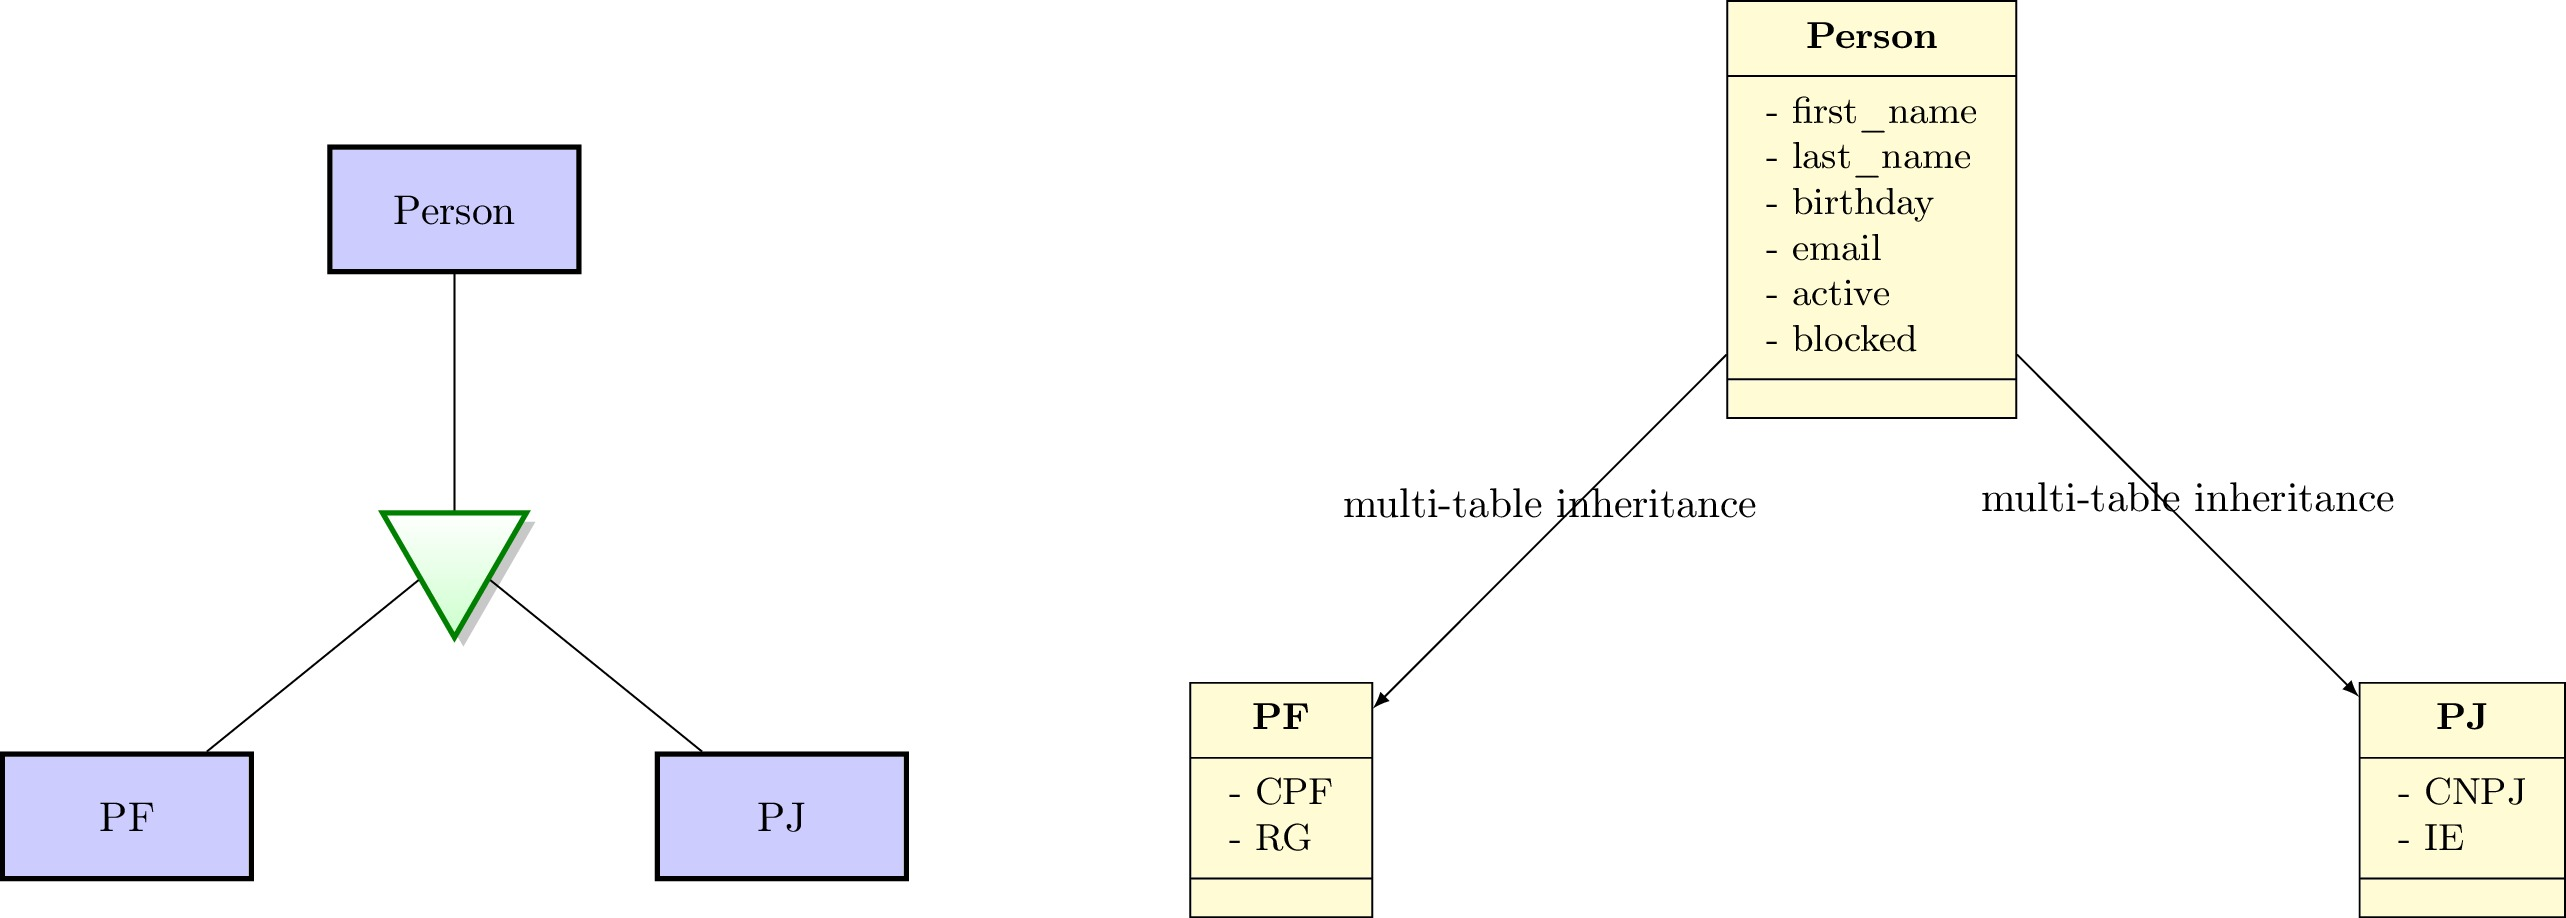
\includegraphics[width=.93\paperwidth]{img/06multitable}
    \end{figure}

\end{frame}

\begin{frame}\frametitle{Multi-table Inheritance (Herança Multi-tabela)}
	
	\begin{figure}[h]
	  \centering
  		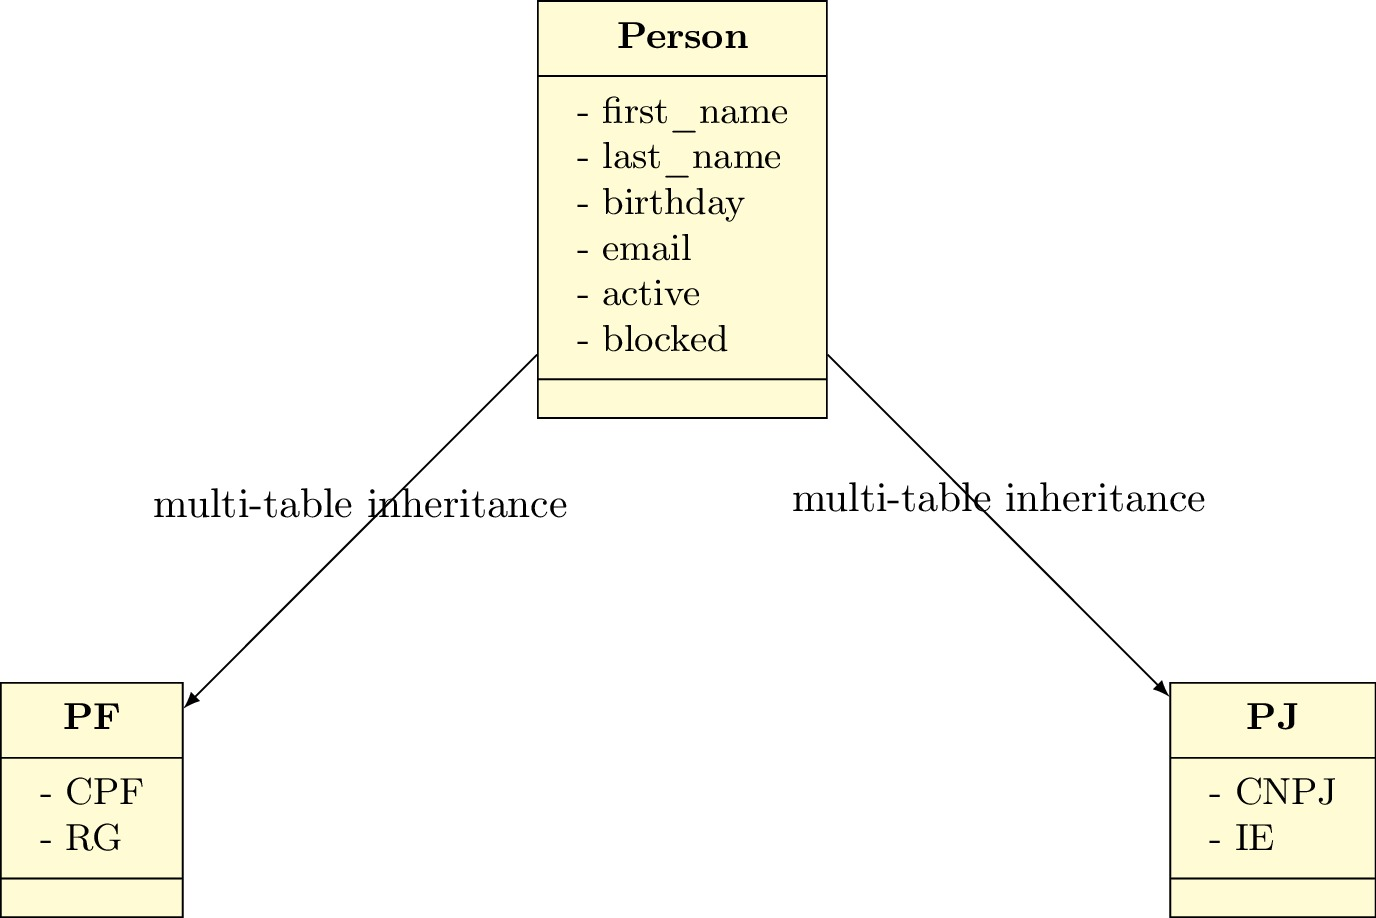
\includegraphics[height=.8\paperheight]{img/061multitable}
	\end{figure}

\end{frame}

\begin{frame}
	
Entrando no banco de dados vemos que a tabela \texttt{core\_pf} possui um campo chamado \texttt{customer\_ptr\_id}....

	\begin{figure}[h]
	  \centering
  		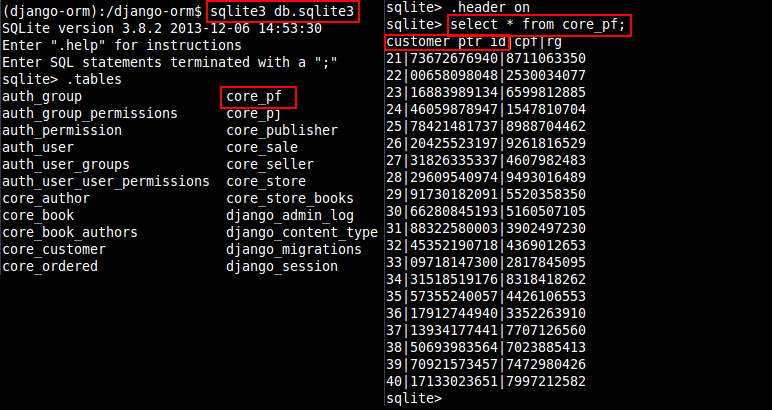
\includegraphics[height=.7\paperheight]{img/core_pf}
	\end{figure}

... e que os ids vão de 21 a 40, neste exemplo.
\end{frame}

\begin{frame}
Note que são os mesmos ids na tabela \texttt{customer}.

	\begin{figure}[h]
	  \centering
  		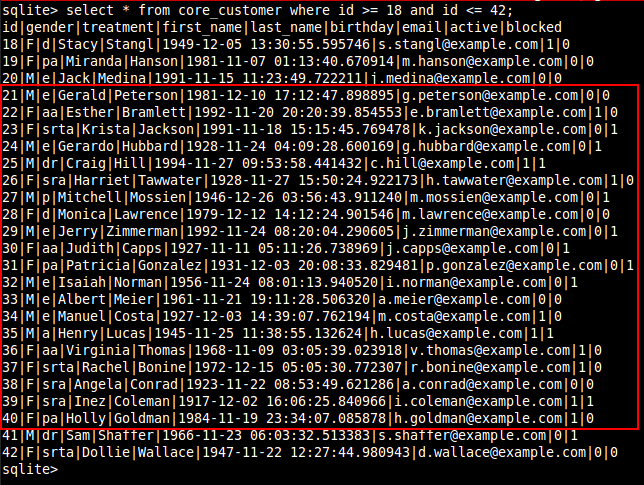
\includegraphics[height=.7\paperheight]{img/customer_table}
	\end{figure}

\end{frame}

\begin{frame}[fragile]
E se você digitar...

\begin{bashcode}
sqlite> .schema core_pf
CREATE TABLE "core_pf" ("customer_ptr_id" 
integer NOT NULL PRIMARY KEY REFERENCES 
"core_customer" ("id"), 
"cpf" varchar(11) NOT NULL, 
"rg" varchar(10) NOT NULL);
\end{bashcode}

\

\

... você verá nitidamente que existe um relacionamento um pra um entre eles.

\end{frame}


\begin{frame}\frametitle{Fixtures}

Vamos criar nossas próprias fixtures usando

\begin{itemize}
	\item Python
	\item csv
	\item shell do Django
\end{itemize}

\end{frame}

\begin{frame}[fragile]\frametitle{random values}
Vamos precisar do \texttt{rstr}.

\

\begin{bashcode}
$ pip install rstr
\end{bashcode}

\url{https://pypi.python.org/pypi/rstr/2.1.3}

\

\

\begin{bashcode}
$ python
>>> import rstr
>>> rstr.rstr('abcde',10)
'ddcbeedacb'
\end{bashcode}

\end{frame}

\begin{frame}[fragile]
	
Apenas uma amostra do poder do Python.

\begin{pythoncode}
# gen_random_values.py
import random
import rstr
import datetime
from decimal import Decimal


def gen_age(min_age=15, max_age=99):
    # gera numeros inteiros entre 15 e 99
    return random.randint(min_age, max_age)
\end{pythoncode}

\end{frame}

\begin{frame}[fragile]

\begin{pythoncode}
def gen_doc(doc='cpf'):
    if doc == 'cpf':
        return rstr.rstr('1234567890', 11)
    elif doc == 'cnpj':
        return rstr.rstr('1234567890', 14)
    elif doc == 'rg':
        return rstr.rstr('1234567890', 10)
\end{pythoncode}	

\end{frame}

\begin{frame}[fragile]
	
\begin{pythoncode}
def gen_phone():
    # gera um telefone no formato (xx) xxxx-xxxx
    return '({0}) {1}-{2}'.format(
        rstr.rstr('1234567890', 2),
        rstr.rstr('1234567890', 4),
        rstr.rstr('1234567890', 4))
\end{pythoncode}

\end{frame}

\begin{frame}[fragile]

\begin{pythoncode}
def gen_timestamp(min_year=1915, max_year=1996):
    # gera um datetime no formato
    # yyyy-mm-dd hh:mm:ss.000000
    year = random.randint(min_year, max_year)
    month = random.randint(11, 12)
    day = random.randint(1, 28)
    hour = random.randint(1, 23)
    minute = random.randint(1, 59)
    second = random.randint(1, 59)
    microsecond = random.randint(1, 999999)
    date = datetime.datetime(
        year, month, day, hour, minute, 
        second, microsecond)
        .isoformat(" ")
    return date
\end{pythoncode}

\end{frame}


\begin{frame}[fragile]
	
\begin{pythoncode}
def gen_decimal(max_digits, decimal_places):
  num_as_str = lambda x: ''.join(
    [str(random.randint(0, 9)) for i in range(x)])
  return Decimal("%s.%s" % (num_as_str(max_digits
                            - decimal_places),
                            num_as_str(decimal_places)))
gen_decimal.required = ['max_digits', 'decimal_places']
\end{pythoncode}

\end{frame}

\begin{frame}[fragile]\frametitle{names}
	
Agora vamos precisar do \texttt{names}.

\

\begin{bashcode}
$ pip install names
\end{bashcode}

\url{https://pypi.python.org/pypi/names/}

\

\begin{bashcode}
$ python
>>> import names
>>> names.get_first_name(gender='male')
'Jean'
>>> names.get_first_name(gender='female')
'Emily'
>>> names.get_last_name()
'Oconnor'
\end{bashcode}

\end{frame}

\begin{frame}[fragile]
	
E vejamos como gerar nomes aleatórios.

\begin{pythoncode}
# gen_names.py
import random
import names
""" List of values for use in choices in models. """
treatment_male_list = ('a','dr','e','p','sr',)
treatment_female_list = ('aa','d','ea','pa','sra','srta',)

def gen_male_first_name():
    treatment = random.choice(treatment_male_list)
    first_name = names.get_first_name(gender='male')
    c = {'treatment': treatment, 'first_name': first_name}
    return c

def gen_female_first_name():
    treatment = random.choice(treatment_female_list)
    first_name = names.get_first_name(gender='female')
    c = {'treatment': treatment, 'first_name': first_name}
    return c

def gen_last_name():
    return names.get_last_name()
\end{pythoncode}

\end{frame}

\begin{frame}[fragile]\frametitle{csv}
	
Para ler um \texttt{csv} façamos o seguinte:

\begin{pythoncode}
import csv

book_list = []

''' Lendo os dados de books_.csv '''
with open('fixtures/csv/books_.csv', 'r') as f:
    r = csv.DictReader(f)
    for dct in r:
        book_list.append(dct)
    f.close()
\end{pythoncode}

\end{frame}

\begin{frame}[fragile]
	
Com isso nós temos uma \textbf{lista} onde os valores são \textbf{dicionários}.

\

\begin{bashcode}
[{'name': 'O diário de Anne Frank', 'publisher': 'Record', 
  'authors': 'Mirjam Pressler'},
 {'name': 'O diário de Anne Frank', 'publisher': 'Record', 
   'authors': 'Otto H. Frank'},
 {'name': 'Deixados Para Trás', 'publisher': 'United Press', 
   'authors': 'Jerry B. Jenkins'},
 {'name': 'Deixados Para Trás', 'publisher': 'United Press', 
   'authors': 'Tim LaHaye'},
 {'name': 'Jardim secreto', 'publisher': 'Sextante', 
   'authors': 'Johanna Basford'},
 {'name': 'Floresta encantada', 'publisher': 'Sextante', 
   'authors': 'Johanna Basford'},
 ...
]
\end{bashcode}

\end{frame}


\begin{frame}[fragile]\frametitle{shell do Django}
	
\begin{bashcode}
$ python manage.py shell
\end{bashcode}

\end{frame}

\begin{frame}[fragile]

O que você precisa saber?

\begin{bashcode}
from core.models import Book, Author, Publisher

''' Criando uma instância do objeto Publisher '''
publisher_obj = Publisher(name='Editora 34',
                          num_awards=8)

''' Salvando o objeto '''
publisher_obj.save()

''' Criando um Author direto com o comando create '''
Author.objects.create(name='Dante Alighieri',
                      age=56)
''' Pegando o id de Author '''
author = Author.objects.get(name='Dante Alighieri')

''' Pegando o id de Publisher '''
publisher = Publisher.objects.get(
    pk=publisher_obj.id)
...
\end{bashcode}
\end{frame}

\begin{frame}[fragile]

\begin{bashcode}
	...
	''' Criando um livro '''
	book_obj = Book(
	    name='A Divina Comédia',
	    publisher=publisher,
	    price=29.20,
	)
	book_obj.save()

	''' Inserindo os autores nos livros '''
	book = Book.objects.get(pk=book_obj.id)

	''' Como o campo authors é ManyToMany devemos usar o comando add '''
	book.authors.add(author)
\end{bashcode}
\end{frame}


\begin{frame}[fragile]

Você pode salvar um arquivo \texttt{shell\_book.py} e digitar

\

\begin{bashcode}
$ ./manage.py shell < fixtures/shell_book.py
\end{bashcode}

\end{frame}


\begin{frame}\frametitle{Vantagens}

\begin{itemize}
	\item Criando o seu próprio código você sabe o que está fazendo
	\item Você vai treinar muito Python
	\item Vai aprender a usar o shell do Django
	\item Fácil de inserir seus próprios dados
\end{itemize}

\end{frame}


\begin{frame}\frametitle{Desvantagens}

\begin{itemize}
	\item Pode demorar um pouco para criar o código
	\item Difícil manutenção
	\item Se fizer uma migração no banco terá que refatorar o código
\end{itemize}

\end{frame}

\begin{frame}\frametitle{Conclusão}

\begin{itemize}
	\item Ninguém recomenda
	\item Recomendam o \href{http://mixer.readthedocs.org/en/latest/index.html}{mixer} ou \href{https://github.com/vandersonmota/model_mommy}{model-mommy}
	\item Mas para inserir seus próprios dados é uma boa solução
\end{itemize}

\end{frame}


\begin{frame}[fragile]
	
Leia o \texttt{Makefile} para ver como foi executado cada comando.

\

Veja a pasta \texttt{fixtures} para ver os códigos Python que geram os valores.
\end{frame}

\begin{frame}
	\centering
	\huge Obrigado!

	\

	\

	\large Dúvidas?
\end{frame}

\begin{frame}
	\titlepage
\end{frame}

\end{document}